\documentclass[12pt,twoside]{article}
\usepackage{jmlda}
\usepackage{tabularx}
%\NOREVIEWERNOTES
\title
    {Раннее прогнозирование достаточного объема выборки для обобщенной линейной модели.}
\author
    {Бучнев~В.\,С., Грабовой~А.\,В., Гадаев~Т.\,Т., Стрижов~В.\,В.} % основной список авторов, выводимый в оглавление


\abstract
    {Исследуется проблема снижения затрат на сбор данных, необходимых для построения
адекватной модели. Рассматриваются задачи линейной и логистической моделей. Для решения этих задач требуется, чтобы выборка содержала необходимое число  объектов. Требуется предложить метод вычисления оптимального обьема данных, соблюдая при этом баланс между точностью модели и и трудозатратами при сборе данных. Предпочтительны те методы оценки объемы, которые позволяют строить адекватные модели по выборкам возможно меньшего объема.

\bigskip
\textbf{Ключевые слова}: \emph {Обобщенная линейная модель, размер выборки}.}
\titleEng
    {JMLDA paper example: file jmlda-example.tex}
\authorEng
    {Author~F.\,S.$^1$, CoAuthor~F.\,S.$^2$, Name~F.\,S.$^2$}
\organizationEng
    {$^1$Organization; $^2$Organization}
\abstractEng
    {This document is an example of paper prepared with \LaTeXe\
    typesetting system and style file \texttt{jmlda.sty}.

    \bigskip
    \textbf{Keywords}: \emph{keyword, keyword, more keywords}.}
\begin{document}
\maketitle
%\linenumbers

\section{Введение}
При планировании эксперимента требуется оценить минимальный объём выборки — число производимых измерений набора показателей или признаков, необходимый для построениие сформулированных условий. 

Существует большое количество оценки размера выборки. Например, тест множителей Лагранжа, тест отношения правдоподобия и тест Вальда. В работах \cite{Self-Mauritsen-1998, Shieh-2000, Shieh-2005} на основе данных методов построена оценка оптимального размера выборки. Основной минус этих методов заключается в том, что статистики, используемые в критериях, имеют асимптотическое распределение и требуют большого обьема выборки.

Существуют также байесовские оценки обьема выборки: критерий средней апостериорной дисперсии, критерий среднего покрытия, критерий средней длины и метод максимизации полезности. Первые три метода требуют анализа некоторой функции эффективности от размера выборки. Используя некоторое решающее правило, по данной функции определяется достаточный объем выборки. Главный минус этих методов заключается в том, что они не позволяют построить аппроксимацию функции эффективности при большем объеме данных. Метод максимизации полезности максимизирует ожидание некоторой функции полезности по обьему выборки. Все эти методы опираются на апостериорное распределение, что требует достаточно большого обьема выборки.

Предлагается исследовать зависимость среднего значения логарифма правдоподобия от размера доступной выборки, а также его дисперсию. В данной работе предлагается использовать не сами функции эффективности, а их аппроксимации. Для этого предлагается использовать аппроксимацию ковариационной матрицы вектора параметров. После чего аппроксимировать данные две зависимости при помощи метода бутстреп. Для вычислительного эксперимента предлагается использовать классические выборки из UCI репозитория и синтетические данные.

\section{Постановка задачи}

Дана выборка размера m:
$$
\mathfrak D_m = \{\textbf{x}_i, y_i\}_{i=1}^m,
$$
где $\textbf{x}_i \in \mathbb{R}^{n}$ - вектор признаков, $~y_i \in \mathbb{Y}$.

Выборка $\mathfrak D_m$ разбита случайно на обучение и контроль:

$$
\mathfrak D_{\mathcal T_m} = \{\textbf{x}_i, y_i\}_{i \in \mathcal T_m} ~~~ \mathfrak D_{\mathcal L_m} = \{\textbf{x}_i, y_i\}_{i \in \mathcal L_m}, ~~~ \mathcal T_m \sqcup \mathcal L_m = \{1, ..., m\}. 
$$

Предполагается, что выборка $\mathfrak D_m$ не противоречит гипотезе порождения данных.

Рассмотрим параметрическое семейство функций для аппроксимации неизвестного распределения $p(y | \textbf{x}, \textbf{w})$, где $\textbf{w} \in \mathbb{W}$ - вектор параметров:

$$
\mathfrak{F} = \left\{f(y, \textbf{x}, \textbf{w}) | \textbf{w} \in \mathbb{W}, \int_{y \in \mathbb{Y}, \textbf{x} \in \mathbb{R}^n} f(y, \textbf{x}, \textbf{w})dyd\textbf{x} = 1\right\}.
$$

Для модели $f$ с вектором параметров $\textbf{w}$ определим функцию правдоподобия и логарифмическую функцию правдоподобия выборки $\mathfrak D$:
$$
L(\mathfrak{D}, \textbf{w}) = \prod_{y, \textbf{x} \in \mathfrak D} f(y, \textbf{x}, \textbf{w}),~~~ l(\mathfrak D, \textbf w) = \sum_{y, \textbf{x} \in \mathfrak D}\log f(y, \textbf{x}, \textbf{w}),
$$
где $f(y, \textbf{x}, \textbf{w})$ - аппроксимация апостериорной вероятности выборки $\mathfrak D_{\mathcal L_m}$ при заданном векторе параметров $\textbf{w}$.

Рассмотрим правдоподобие выборки $\mathfrak D_{\mathcal L_m}$:

$$
L(\mathfrak D_{\mathcal T_m}, \mathfrak D_{\mathcal L_m}) = \prod_{y, \textbf{x} \in \mathfrak D_{\mathcal T_m}} f(y, \textbf{x},  \textbf{w}).
$$

Рассмотрим логарифм правдоподобия выборки $\mathfrak D_{\mathcal L_m}$:

$$
l(\mathfrak D_{\mathcal T_m}, \textbf w) = \sum_{y, \textbf{x} \in \mathfrak D_{\mathcal T_m}}\log f(y, \textbf{x}, \textbf{w}).
$$

Будем рассматривать ожидаемое значение функции $l$:

$$
\tilde{l}(\mathfrak D)  = \underset{y, \textbf{x} \in \mathfrak D}{\mathsf E} l(\{y, \textbf{x}\}, \textbf w).
$$

Рассмотрим ожидаемое значение логарифма правдоподобия по разным обучающим выборкам $\mathfrak D_{\mathcal L_m}$ размера $m^*$:

$$
l(m^*) = \underset{\mathfrak D_{\mathcal L_m}}{\mathsf E} \tilde{l}(\mathfrak D_{\mathcal L_m}).
$$

Будем считать, что объем выборки достаточный, если:

$$
\forall m_1, m_2 > m^* ~~~ |l(m_1) - l(m_2)| < \epsilon,
$$
где $\epsilon$ - достаточно малое пороговое значение.


Для оценки вектора параметров используется принцип максимума правдоподобия:

$$
\hat{\textbf{w}} = \argmax_{\textbf{w} \in \mathbb{W}} L(\mathfrak D_{\mathcal L_m}, \textbf{w}).
$$

Рассмотри матрицу информации Фишера:

$$
\textbf{I}(\mathfrak D, \textbf{w}) = -\nabla\nabla l(\mathfrak D, \textbf{w}).
$$

Будем считать, что $\hat{\textbf{w}}$ имеет следующее распределение:

$$
\hat{\textbf{w}} \sim \mathcal{N}(\textbf{m}, \textbf{V}),~~~ \textbf{V} = \textbf{I}^{-1}(\mathfrak D, m).
$$

Для линейной регрессии $\mathbb{Y} = \mathbb{R}$, где $y$ представимо в виде:

$$
y = \textbf{x}^{\top}\textbf{w} + \epsilon,
$$
где $\epsilon \sim \mathcal{N}(0, 1)$. 

Аппроксимация плотности апостериорной вероятности имеет вид:

$$
f(y, \textbf{x}, \textbf{w}) = \mathcal{N}(y|\textbf{x}^{\top}\textbf{w}, 1).
$$ 

Для логистической регрессии $\mathbb{Y} = \{0, 1\}$, где $y$ является бернуллиевской случайной величиной:

$$
y \sim \mathcal{B}e(\theta),
$$
где $\theta$ - неизвестный параметр распределения. Аппроксимация плотности апостериорной вероятности имеет вид:

$$
f(y, \textbf{x}, \textbf{w}) = \mathcal{B}e(y|\theta),~~~ \theta = \frac{1}{1 + exp(-\textbf{x}^{\top}\textbf{w})}.
$$

\section{Анализ эффективности модели}

Методы байесовских оценок объема выборки основаны на ограничении некоторой выбранной характеристики модели. Для анализа эффективности вводится функция от объема выборки, увеличение значений которой интерпретируется как уменьшение эффективности модели. Объем выборки $m^{*}$ выбирается таким, при котором исследуемая функция не превышает некоторого порогового значения $\epsilon$.

\subsection{Критерий средней длины}

Пусть $A(\mathfrak{D}) \subset \mathbb{R}^n$ --- множество значений параметров модели \textbf{w}:

$$
A(\mathfrak{D}) = \{\textbf{w} : ||\textbf{w}- \hat{\textbf{w}}|| \leqslant \alpha\}
$$
такое, что
$$
\mathsf{P}(A(\mathfrak{D})) = 1 - \alpha,
$$
где $\alpha$ --- некоторое малое значение. 

Критерий средней длины выглядит следующим образом:

$$
\forall m \geqslant m^{*}~\mathsf{E}_{\mathfrak D_m} r_m \leqslant l , 
$$
где $r_m$ --- радиус шара $A(\mathfrak{D}_m)$, $l$ --- некоторое наперед заданное достаточно малое значение.

\section{Вычислительный эксперимент}

Для анализа точности и эффективности предлагаемого метода был проведен вычислительный эксперимент. В качестве данных использовались выборки, описанные в таблице 1.

\begin{table}[h!]
\begin{center}
\caption{Описание выборок}
\label{table2}
\begin{tabularx}{\textwidth}{|p{1in}|X|X|c|}
\hline
	\centering Выборка &\centeringТип задачи&\centering Размер выборки& Число признаков\\
	\hline
	Servo &регрессия&\centering167&4\\
	\hline
	Boston &регрессия&\centering506&13\\
	\hline
	Diabetes&регрессия&\centering 442&5\\
\hline
\end{tabularx}
\end{center}
\end{table}

В ходе эксперимента был модифицирован критерий средней длины для линейной регрессии, а именно была построена аппроксимация функции эффективности при большем объеме выборки при помощи аппроксимации ковариационной матрицы вектора параметров через матрицу информации Фишера.

\begin{figure}[h!t]\center
\subfloat[Servo]{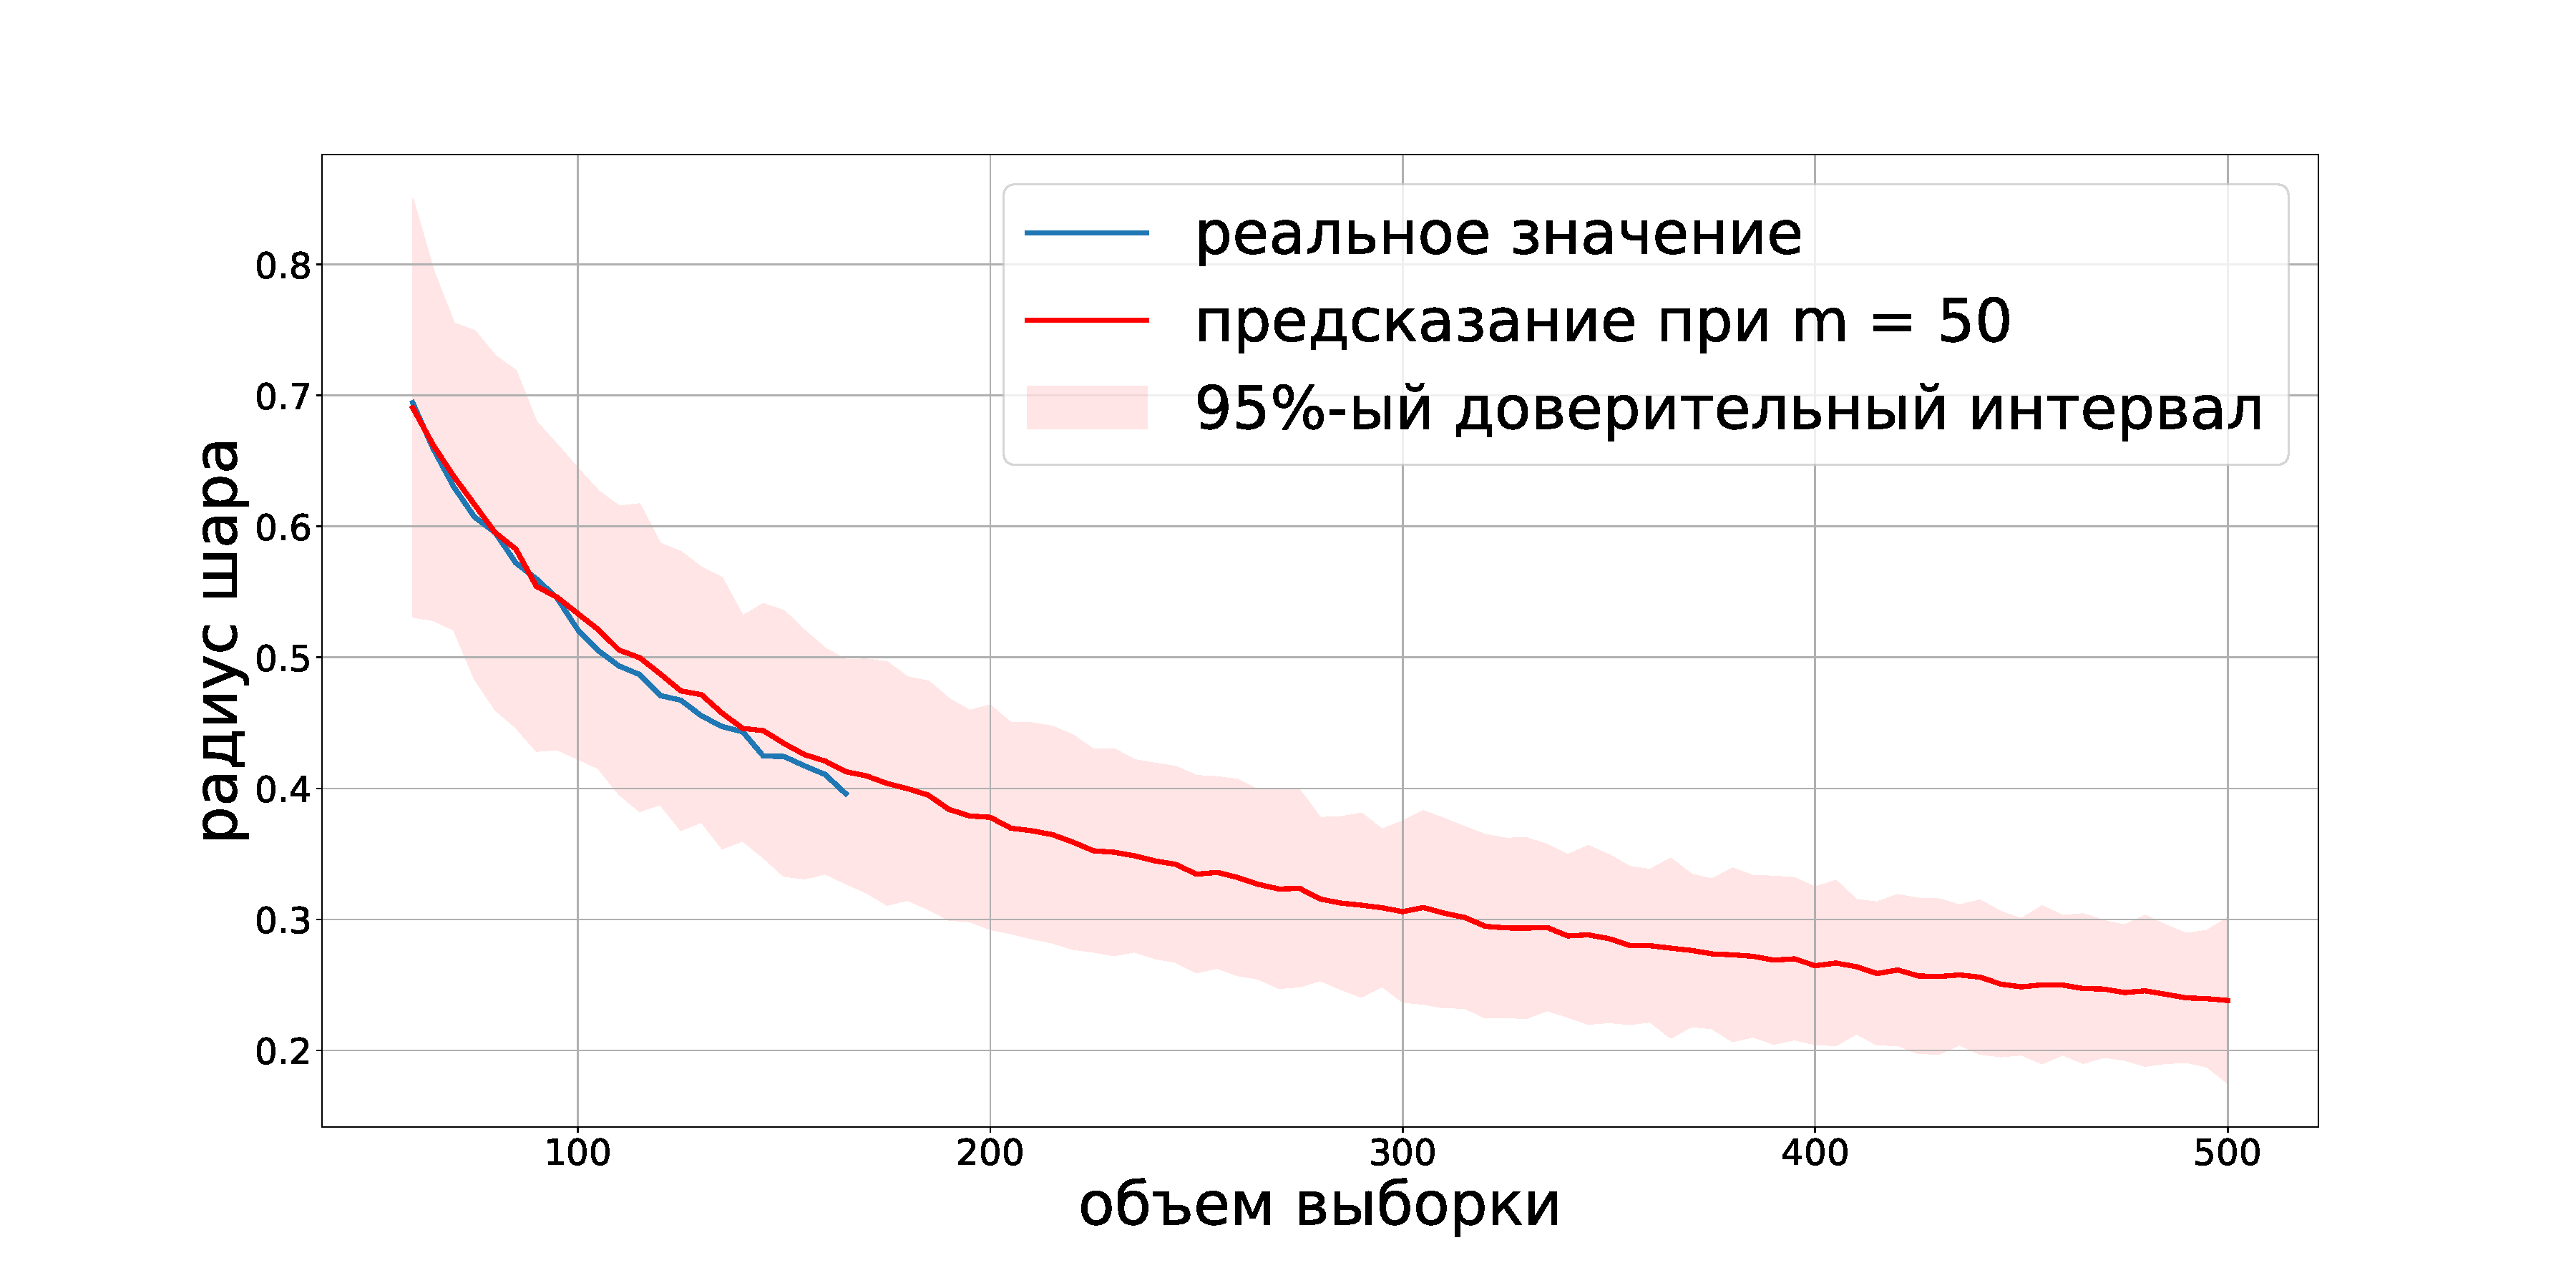
\includegraphics[width=0.5\textwidth]{../data/pics/ALC_modified_servo.pdf}}
\subfloat[Boston]{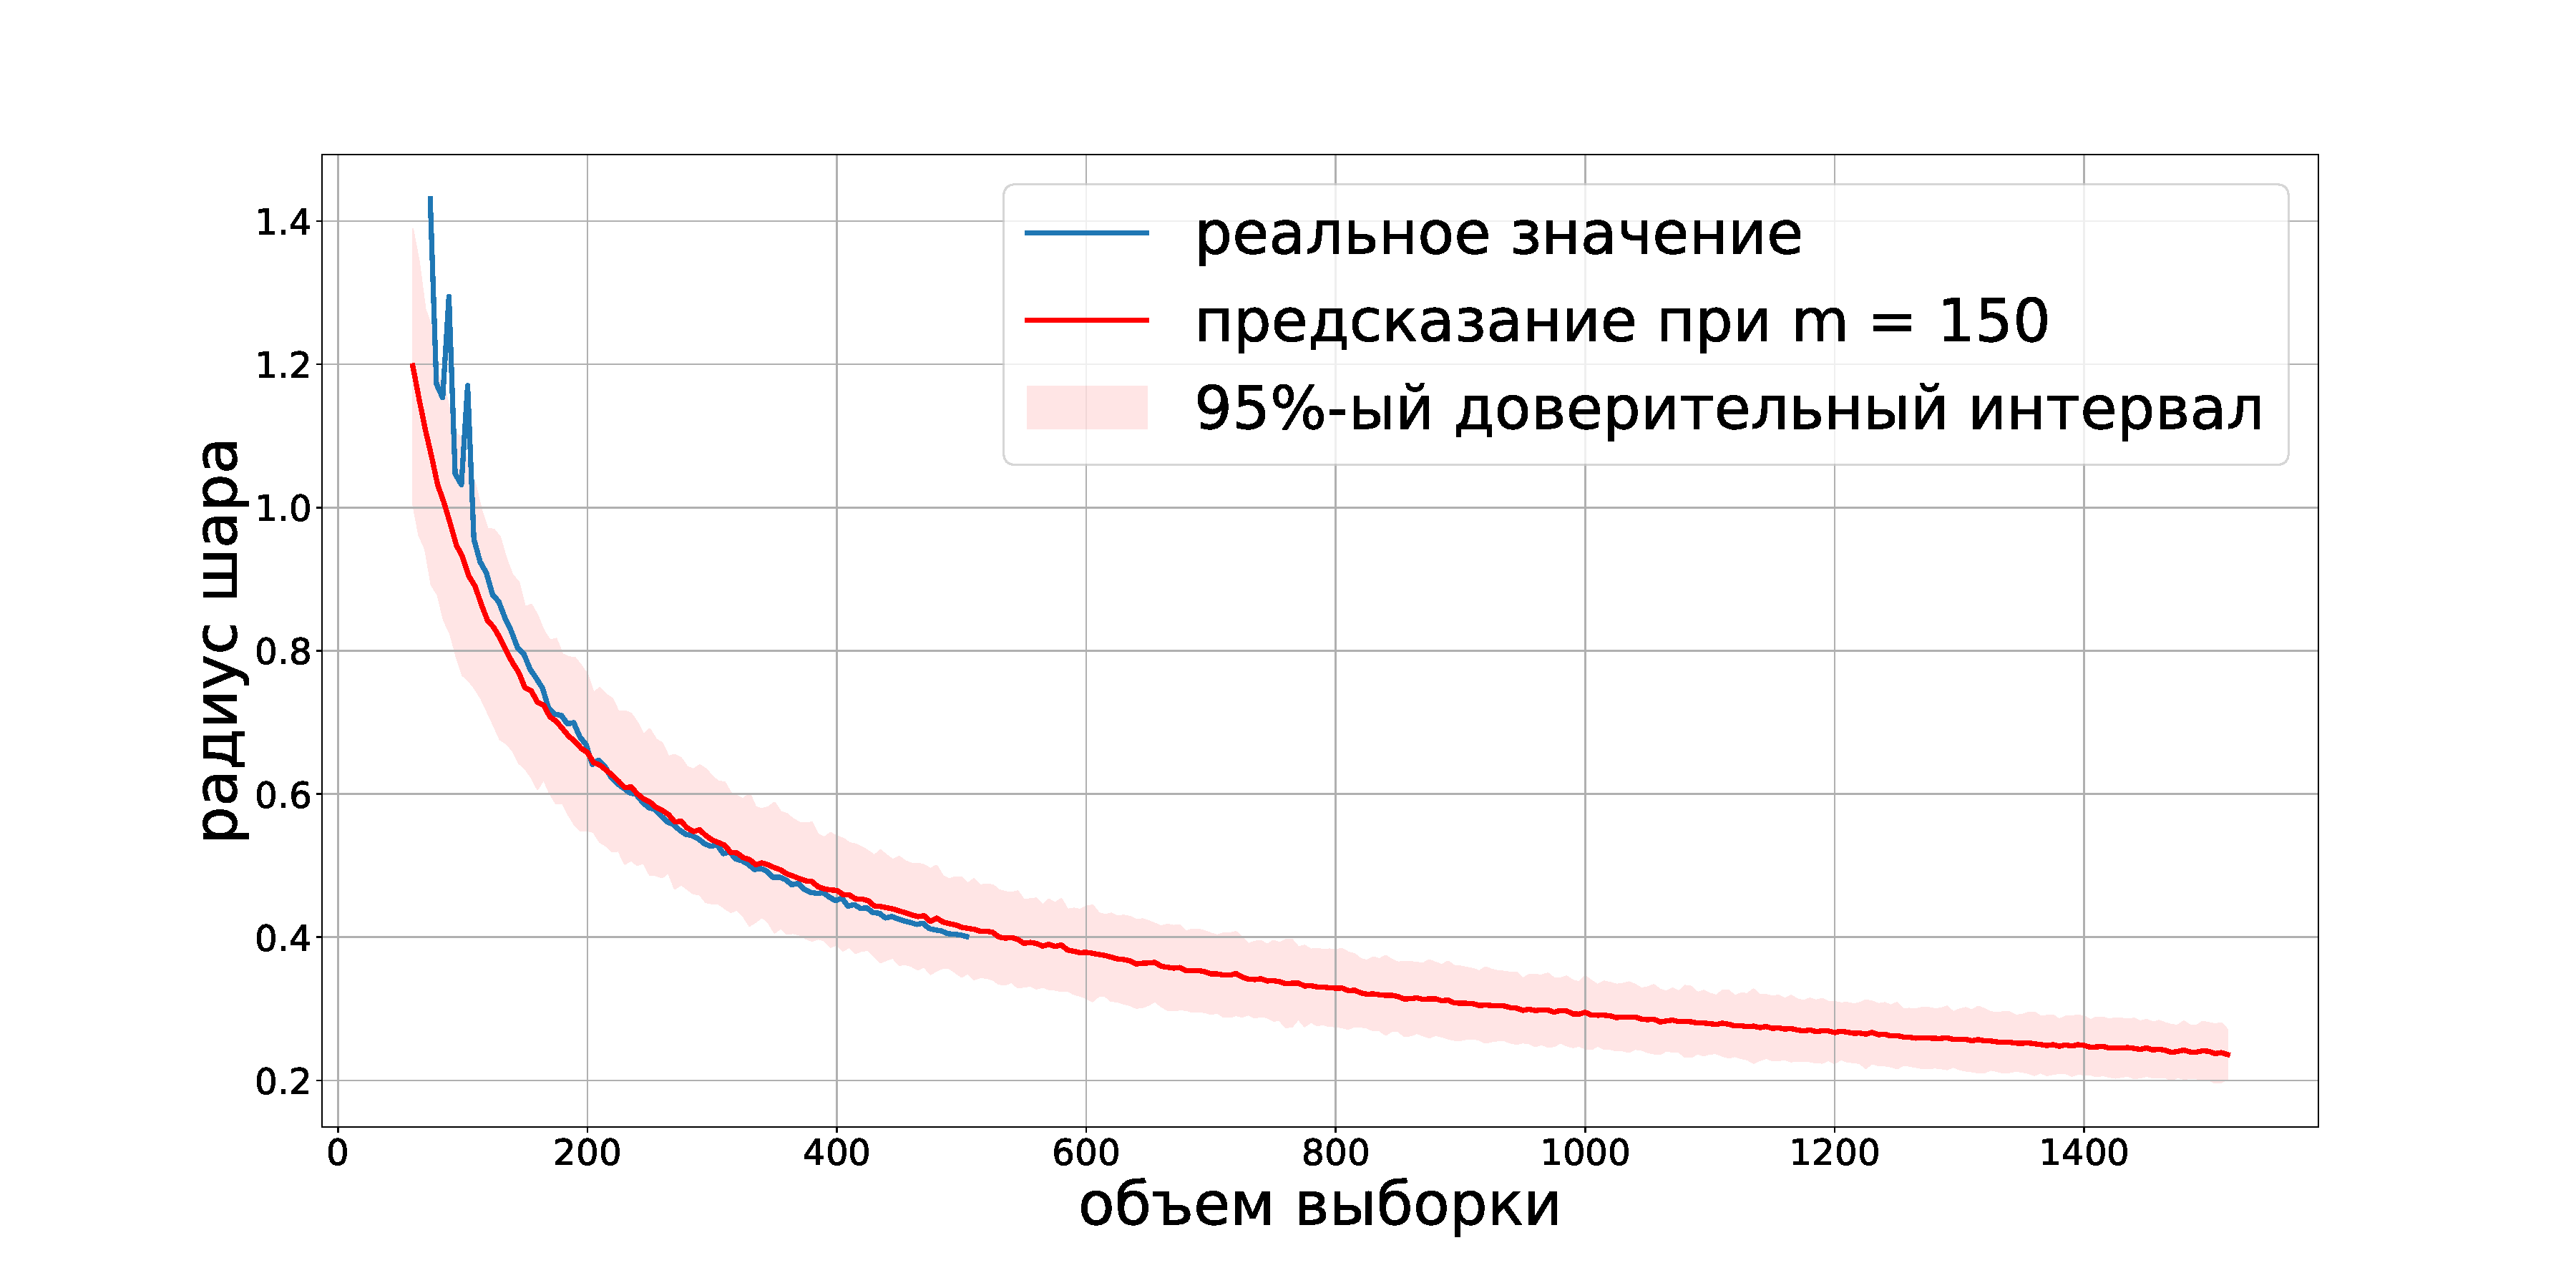
\includegraphics[width=0.5\textwidth]{../data/pics/ALC_modified_boston.pdf}}\\
\subfloat[Diabetes]{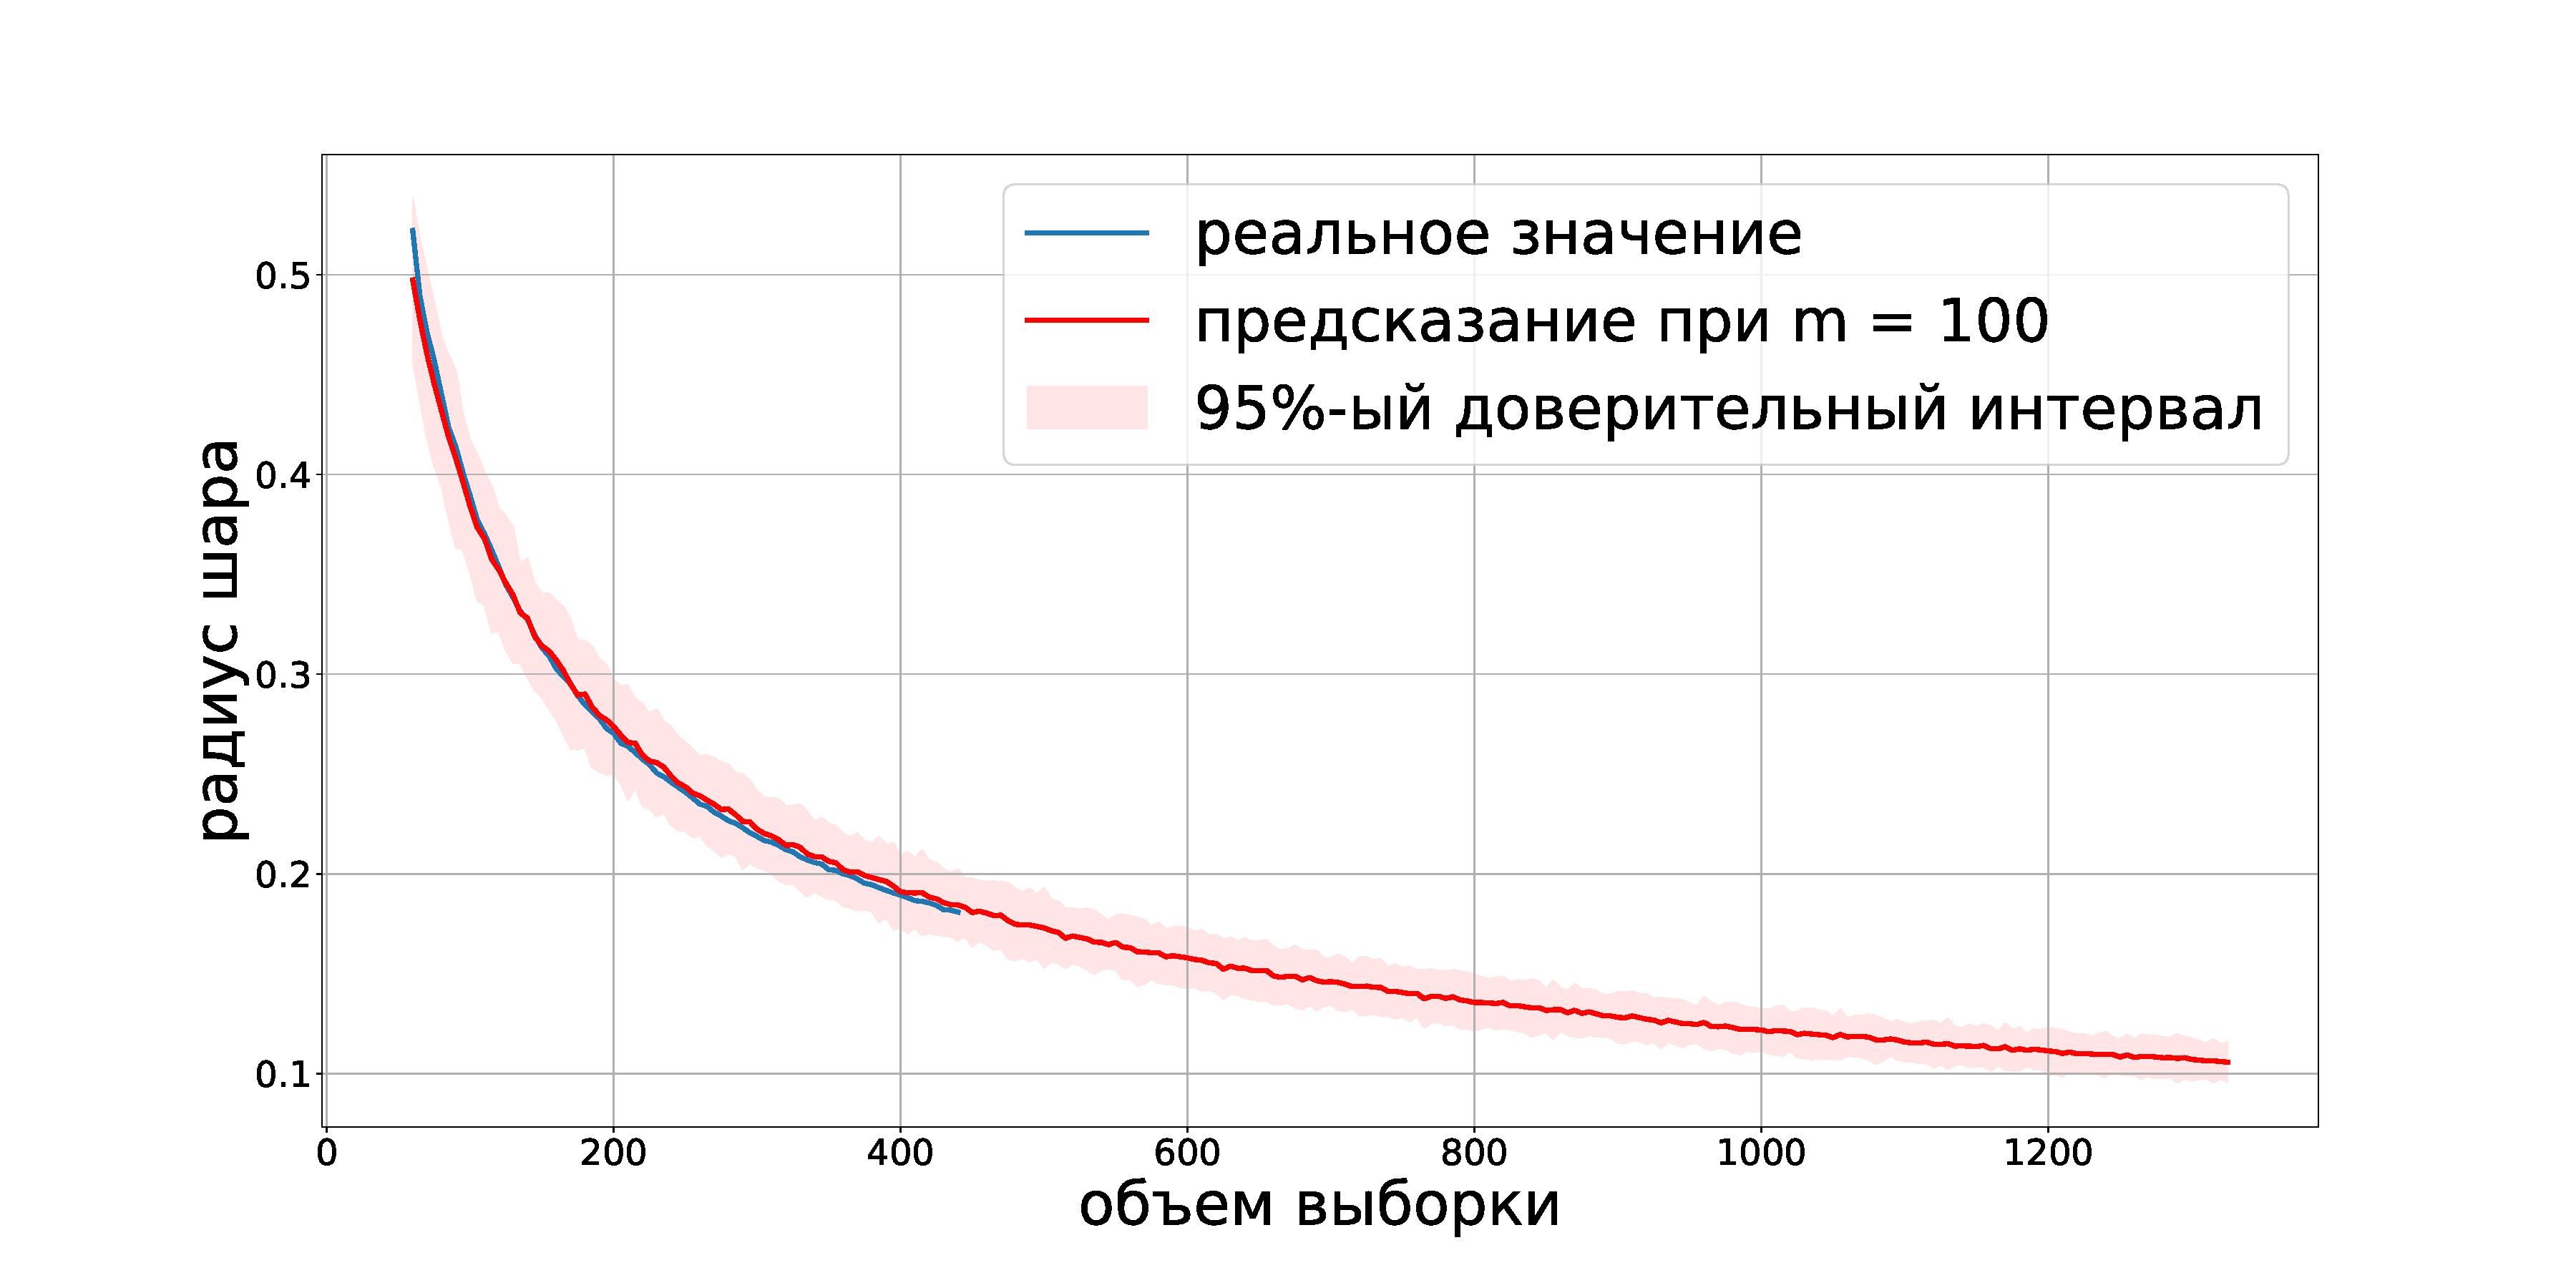
\includegraphics[width=0.5\textwidth]{../data/pics/ALC_modified_diabetes.pdf}}\\

\caption{ACC метод}
\label{fig1}
\end{figure}

На графике 1 показана зависимость значения функции эффективности от объема выборки при разных данных. Синим цветом обозначено посчитанное значение при данном объеме, красным - аппроксимация при подвыборке фиксированного размера. Реальное значение функции эффективности попадает в доверительный интервал, что говорит о работоспособности метода.

\bibliographystyle{unsrt}
\bibliography{jmlda-bib}
\begin{thebibliography}{1}


\bibitem{Self-Mauritsen-1998}
\BibAuthor{S.\,G.\;Self and R.\,H.\;Mauritsen}
\BibTitle{Power/sample size calculations for generalized linear
models }~//
\BibJournal{Biometrics}, 1988.

\bibitem{Shieh-2000}
\BibAuthor{G.\,Shieh}
\BibTitle{On power and sample size calculations for likelihood ratio tests in generalized
linear models}~//
\BibJournal{Biometrics}, 2000.

\bibitem{Shieh-2005}
\BibAuthor{G.\,Shieh}
\BibTitle{On power and sample size calculations for Wald tests in generalized linear
models}~//
\BibJournal{Journal of Statistical Planning and Inference}, 2005.


\bibitem{Rubin-Stern-1998}
\BibAuthor{D.\,B.\;Rubin and H.\,S.\;Stern}
\BibTitle{Sample size determination using posterior predictive
distributions }~//
\BibJournal{Sankhya : The Indian Journal of Statistics Special Issue on Bayesian
Analysis}, 1998.

\bibitem{Qumsiyeh-1998}
\BibAuthor{Maher Qumsiyeh}
\BibTitle{Using the bootstrap for estimation the sample size in statistical
experiments }~//
\BibJournal{Journal of modern applied statistical methods}, 2002.

\end{thebibliography}

\end{document}
